\documentclass[a4paper, 8pt, oneside]{article}

 \usepackage[margin=1in]{geometry} 
\usepackage{amsmath,amsthm,amssymb, float,centernot}
\usepackage[shortlabels]{enumitem}
 \usepackage[hidelinks]{hyperref}
\usepackage{xcolor}
\hypersetup{
    colorlinks,
    linkcolor={red!50!black},
    citecolor={blue!50!black},
    urlcolor={blue!80!black}
}
\usepackage{tikz}
\usepackage{graphicx}
\newtheorem{theorem}{Theorem}[section]
  
\newcommand{\N}{\mathbb{N}}
\newcommand{\Z}{\mathbb{Z}}
\newcommand{\R}{\mathbb{R}}
\newcommand\abs[1]{\left|#1\right|}
\newenvironment{sol}
    {\emph{Solution:}
    }
    {
    \qed
    }
\begin{document}

\title{Computational Geometry: Assignment 3}
\author{Oren Friman 301677613}
\maketitle

\medskip

\begin{enumerate}
\item Attached.
\item Prove that any algorithm for the shortest homotopic curve problem must run in time $\Omega(n\log n + kn)$ in the worst case.

\begin{sol}
Proof by contradiction using reduction.  \\
Assume that there is Algorithm $A$ for the shortest homotopic curve problem that run in $T(A)$ and is smaller than $\Omega(n\log n + kn)$ in the worst case.
We will use Algorithm $A$ to solve the sorting problem in $\mathcal{O}(T(A))$ . \\

Sorting Problem: \\
Input: $x_1, \ldots, x_n$ \\
Output: input ordered \\
Algorithm:\\
$obstacles = (x_1, x_1^2), \ldots, (x_n, x_n^2)$ \\
$path =  (x_1, x_2, x_3, x_4)$ such that the path is rectangle that contain all obstacles inside him.\\
$CH = A(obstacles, path)$ \\
we will iterate over $CH$ and we will return those points from the smallest x-coordinate in asc order.
\begin{figure}[h]
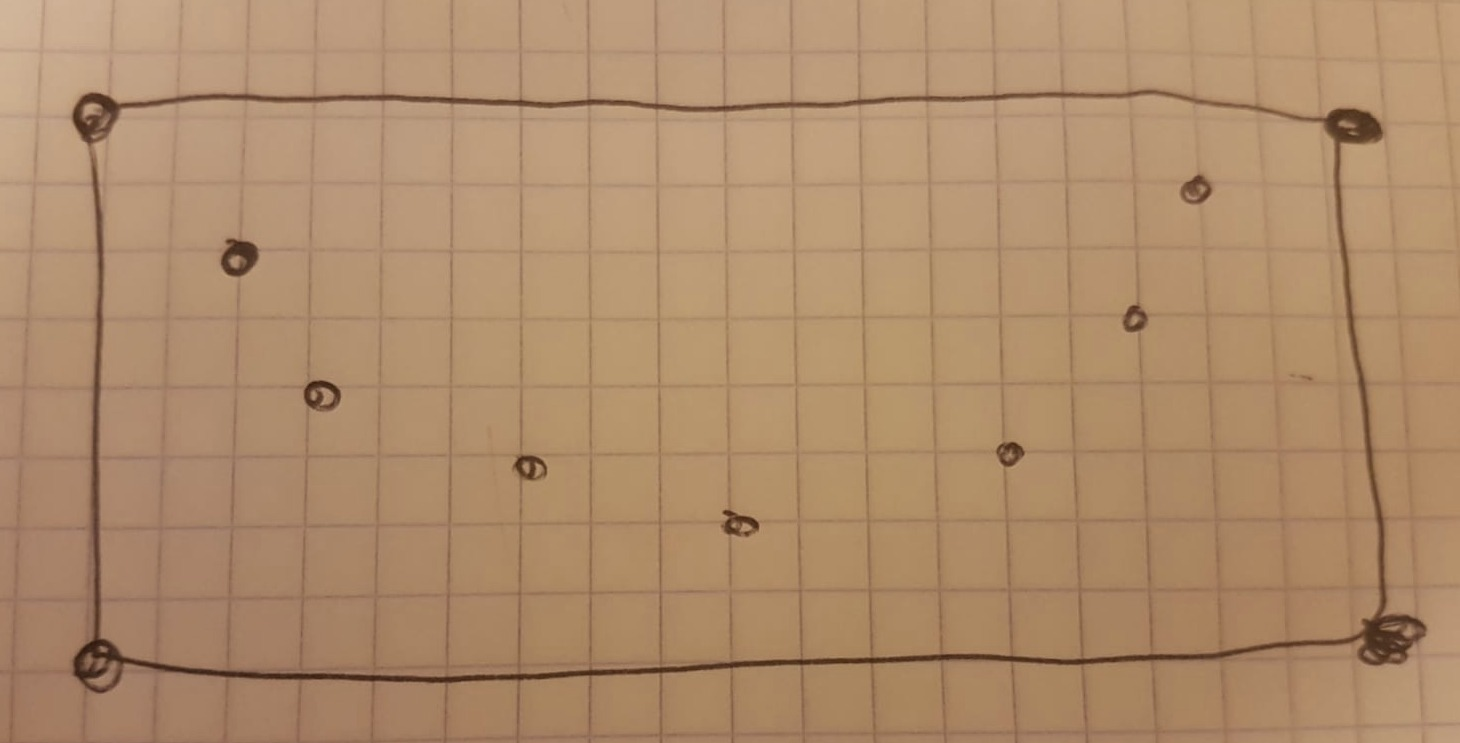
\includegraphics[scale=0.1]{parabola}
\centering
\end{figure} \\
Correctness: notice that the path (curve) contain the obstacles (points in parabola) inside him (without any intersections with the Convex Hull of the obstacles)

and so the smallest homotopic curve will be the Convex Hull of the obstacles that by definition contain the points sorted \\

Time analysis: $\mathcal{O}(n) + T(A)$. \\

$\mathcal{O}(n)$  - iterating over the obstacle once and calculate each point in the obstacle $(x_i, x_i^2)$ and saving min and max for each axis, after the loop we can use the min and max to define the path.\\
$T(A)$ -  running A. \\
Notice that k = len(path) = 4 $T(A) < \Omega(n\log n + 4n)$

\end{sol}
\end{enumerate}
\end{document}